
\section{基础知识}

基于视频序列的运动目标检测与跟踪涉及到很多研究领域,如数字图像处理、计算机视觉、信息融合、模式识别与人工智能等。

\subsection{视频图像预处理}

\subsubsection{常用颜色模型}

颜色模型的用语是在某些标准下用通常可接受的方式简化彩色规范。本质上颜色模型是坐标系统和子空间的规范。位于系统中的每种颜色都由单个点来表示。

(1)~RGB彩色模型:

在RGB模型中,每种颜色出现在红、绿、蓝的原色光谱分量中,这个模型基于笛卡尔坐标系。

图\ref{fig:RGB彩色立方体示意图}所示的立方体。图中R、G、B位于$3$个角上。在该模型中,灰度等级沿着主对角线从原点的黑色到点$(1,1,1)$的白色分布。
\begin{figure}[H]
  \centering
  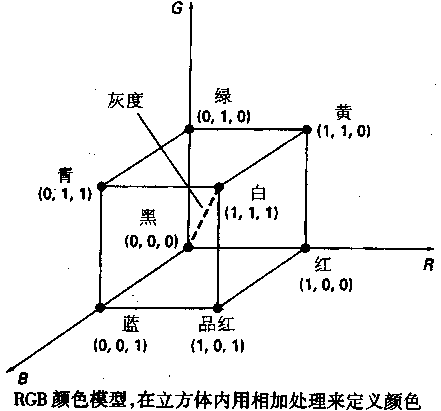
\includegraphics[width=0.45\textwidth]{STEM/fig_ch2/RGB彩色立方体示意图.png}
  \caption{RGB彩色立方体示意图}
  \label{fig:RGB彩色立方体示意图}
\end{figure}

(2)~灰色模型:

本质上颜色模型是坐标系统和子空间的规范。位于系统中的每种颜色都由单个点来表示。单位在每列的书写示例如表\ref{tab:单位在每列的书写示例}所示。

\begin{table}[H]
  \centering
  \caption{单位在每列的书写示例}
    \begin{tabular}{ccccc}
    \toprule
    基体 & 序号 & \makecell[c]{粉末类型和\\ 预热温度(\unit{\degreeCelsius})} & 失效温度(\unit{\degreeCelsius}) & $E_c$计算值(\unit{\GPa})\\
    \midrule
    \multicolumn{1}{c}{\multirow{4}[2]{*}{SUS304不锈钢}} & 1     & 粗粉 \& 1000 & 180   & 4.21 \\
          & 2     & 粗粉 \& 800 & 10    & 4.38 \\
          & 3     & 细粉 \& 1000 & 300   & 4.95 \\
          & 4     & 细粉 \& 800 & 120   & 5.08 \\
    \bottomrule
    \end{tabular}%
  \label{tab:单位在每列的书写示例}%
\end{table}%

表格的分栏情况示例如表\ref{tab:分栏情况示例}所示。
% Table generated by Excel2LaTeX from sheet 'Sheet1'
\begin{table}[H]
  \centering
  \caption{分栏情况示例}
    \begin{tabular}{cccc}
    \toprule
    \multicolumn{1}{c}{基体} & 粉末类型 & \multicolumn{1}{c}{预热温度(\unit{\degreeCelsius})} & \multicolumn{1}{c}{平均值} \\
    \midrule
    \multicolumn{1}{c}{\multirow{6}[4]{*}{SUS304不锈钢}} & \multirow{3}[2]{*}{粗粉} & 600   & 44.28\% \\
          & \multicolumn{1}{c}{} & 800   & 42.37\% \\
          & \multicolumn{1}{c}{} & 1000  & 39.74\% \\
\cmidrule{2-4}          & \multirow{3}[2]{*}{细粉} & 600   & 27.95\% \\
          & \multicolumn{1}{c}{} & 800   & 25.41\% \\
          & \multicolumn{1}{c}{} & 1000  & 24.77\% \\
    \midrule
    \multicolumn{1}{c}{\multirow{2}[2]{*}{碳钢}} & 粗粉    & 1000  & 35.65\% \\
          & 细粉    & 1000  & 22.95\% \\
    \bottomrule
    \end{tabular}%
  \label{tab:分栏情况示例}%
\end{table}%

表的通栏情况和全表统一单位的情况如表\ref{tab:插入表格的通栏示例(单位:台)}所示。
% Table generated by Excel2LaTeX from sheet 'Sheet1'
\begin{table}[htbp]
  \centering
  \caption{插入表格的通栏示例(单位:台)}
    \begin{tabular}{cccc}
    \hline%\toprule
    \diagbox{时间}{地点} & 电风扇 & 冰箱 & 洗衣机 \\
    \hline%\midrule
    10月   & 100   & 200   & 300 \\
    11月   & 200 & & \\
    12月   & 200 & 100   & 400 \\
    \hline%\midrule
    合计    & 500   & 500   & 900 \\
    \hline%\bottomrule
    \end{tabular}%
  \label{tab:插入表格的通栏示例(单位:台)}%
\end{table}%

{\color{red}\lipsum[4]} %添加这么一段测试文本是为了展示跨页表格的效果

若表格一页内放不下,可以使用跨页表格。跨页表格的情况如表\ref{tab:CMS_VIDEO数据表(跨页表格)}所示。
\begin{longtable}{ccccc}
    \caption{CMS\_VIDEO数据表(跨页表格)} \label{tab:CMS_VIDEO数据表(跨页表格)} \\
	\toprule
	字段标识 & 字段含义 & 数据类型 & 是否主键 & 是否外键 \\
	\midrule
    \endfirsthead %以上是首页表头
    \caption{(续表)} \\ %续表对应的标题
    \midrule
    字段标识 & 字段含义 & 数据类型 & 是否主键 & 是否外键 \\
    \midrule
    \endhead %以上是通用表头
    \midrule
    \endfoot %以上是通用表尾
    \bottomrule
    \endlastfoot %以上是末页表尾,以下是表格正文
    ID & ID & INTEGER & 是 & 否 \\
    VIDEO\_NAME & 视频名称 & VARCHAR2($20$) & 否 & 否 \\
    VIDEO\_TYPE & 视频类型 & VARCHAR2($20$) & 否 & 是 \\
    VIDEO\_PATH & 视频路径 & VARCHAR2($20$) & 否 & 否 \\
    UPLOADER\_ID & 上传人ID & INTERGER & 否 & 是 \\
    UPLOAD\_DATE & 上传日期 & DATE & 否 & 否 \\
    ISPASS & 是否审批 & INTERGER & 否 & 否
\end{longtable}

\subsection{本章小结}

本章主要介绍了表格的显示。